\documentclass{beamer}
\usetheme{Madrid}
\usepackage[utf8]{inputenc}
\usepackage{default}
\usepackage{graphicx}
\usepackage{hyperref}

\title{ASSR: Automatic Stuttered Speech Recognition}
\author{Anshul Gupta}
\institute{IIT Bombay}
\date{\today}

\begin{document}
\begin{frame}
\titlepage
\end{frame}

\begin{frame}
\frametitle{Introduction}
\begin{enumerate}
 \item More than 70 million people worldwide are stutterers -- that's one in every 100
 \item State of the art speech-to-text systems fails miserably with accuracy as low as 18\% and as high as 73\% as compared to a baseline of 92\% for normal speaker \cite{siriStats}
 \item The existing work \cite{manuChopra} that has been done for this problem is just classification of a speech as a stuttered speech or a normal speech
\end{enumerate}
\end{frame}

\begin{frame}
\frametitle{Dataset}
\begin{enumerate}
 \item University College London Archive of Stuttered Speech (UCLASS) \cite{uclass} database
 \item Recordings of monologues, reading and conversations of different speakers ranging from 7 to 20 years old
 \item Most of them do not have time aligned labels and/or orthographic transcriptions
 \item We are using 16 audio files have time aligned labels
 \item .wav files having sampling rate of 22050Hz
\end{enumerate}

\end{frame}

\begin{frame}
\frametitle{Methodology}
\begin{figure}[ht]
    \centering
    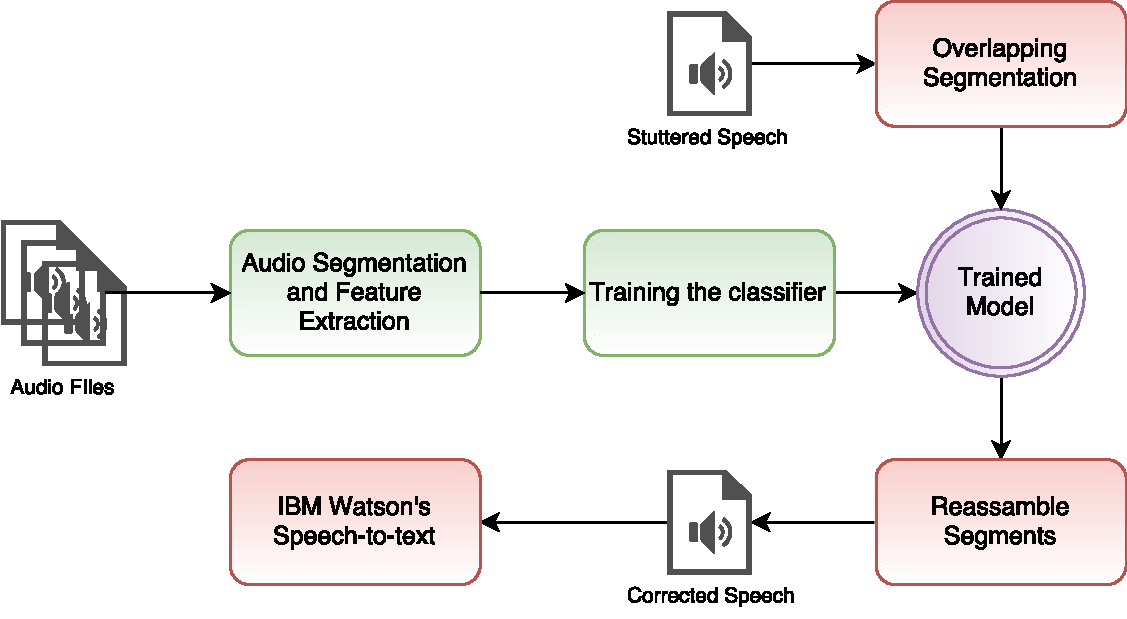
\includegraphics[scale=0.60]{FlowDiagram.pdf}
    \caption{Flow Diagram}
    \label{fig:flowdiagram}
\end{figure}

\end{frame}

\begin{frame}[allowframebreaks]
\frametitle{Methodology: Data Pre-processing}
Used the time-aligned transcriptions to split the data files into stuttered segments and normal segments
\begin{table}[ht]
\centering
\caption{Data Statistics}
\label{table:data-statistics}
\begin{tabular}{|l|r|r|r|}
\hline
                     & \multicolumn{1}{l|}{\textbf{ALL}} & \multicolumn{1}{l|}{\textbf{STUTTER}} & \multicolumn{1}{l|}{\textbf{NORMAL}} \\ \hline
\textbf{COUNT}       & 12633                             & 2643                                  & 9990                                 \\ \hline
\textbf{MAX (ms)}    & 17044                             & 17044                                 & 14499                                \\ \hline
\textbf{MIN (ms)}    & 0                                 & 1                                     & 0                                    \\ \hline
\textbf{MEAN (ms)}   & 315.0925                          & 762.5323                              & 196.7158                             \\ \hline
\textbf{MEDIAN (ms)} & 192                               & 486                                   & 168                                  \\ \hline
\textbf{MODE (ms)}   & 109                               & 201                                   & 93                                   \\ \hline
\end{tabular}
\end{table}
\break
\begin{enumerate}
 \item Very unlikely to see a 17 sec stuttered segment
 \item We Segmented the files segments further down to less than or equal to 300 ms
 \item This segmentation created 17,545 segments which were used for training the models
\end{enumerate}


\begin{figure}[ht]
    \centering
    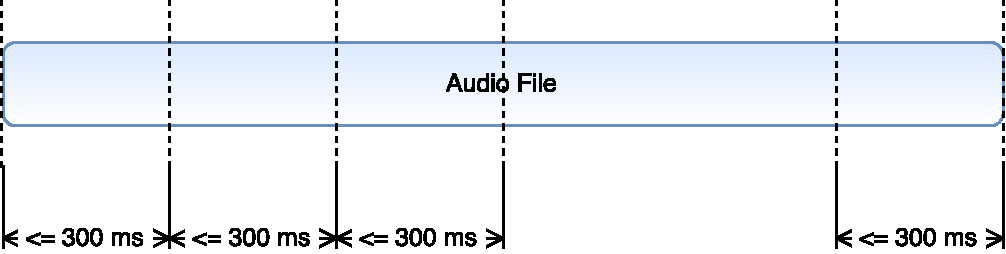
\includegraphics[scale=0.7]{AudioSplits300ms.pdf}
    \caption{Audio segments}
    \label{fig:audioSegments}
\end{figure}
\end{frame}

\begin{frame}
\frametitle{Methodology: Feature Extraction}
\begin{enumerate}
 \item MFCC features as they are very representative of human speech
 \item RMSE which represents the loudness of a speech
 \item Feature vector had mean and variance of 39 + 1 features
 \item Overall 80 features
\end{enumerate}
\end{frame}

\begin{frame}
\frametitle{Methodology: Classification}
\begin{enumerate}
 \item DNN gave the highest accuracy and took around $\sim$1 min to train as compared with SVC which took more than 1.5 hours.

 \item DNN had 3 hidden layers, each having 10 neurons. Learning rate was 0.001 and training epochs were 1,200
\end{enumerate}
\begin{table}[ht]
\centering
\caption{Classification Accuracy of models}
\label{table:classificationAccuracy}
\begin{tabular}{|l|r|}
\hline
                                   & \multicolumn{1}{l|}{\textbf{Accuracy (\%)}} \\ \hline
\textbf{DNN}                       & 87.07\%                                     \\ \hline
\textbf{SVC}                       & 85.43\%                                     \\ \hline
\textbf{Decision Trees}            & 76.63\%                                     \\ \hline
\textbf{Gaussian Na\"ive Bayes}    & 76.63\%                                     \\ \hline
\textbf{Bernoulli Na\"ive Bayes}   & 71.43\%                                     \\ \hline
\textbf{Multinomial Na\"ive Bayes} & 71.43\%                                     \\ \hline
\end{tabular}
\end{table}
\end{frame}

\begin{frame}
\frametitle{Methodology: Audio Correction}
With the classifier trained with an accuracy of $\sim$87\%, next in the pipeline is audio correction.
\end{frame}

\begin{frame}[allowframebreaks]
\frametitle{Audio Correction: Overlapping Segmentation}
\begin{enumerate}
 \item Model is trained on audio segments of duration $<=$ 300ms
 \item It was only obvious that the audio to be corrected needs to be segmented with duration of 300ms
 \item Less obvious was to detect the stutter boundaries
 \item Instead of na\"ively segmenting the audio in contiguous manner, we overlapped the segments
 \item We could detect the stuttered and non-stuttered parts with the granularity of 100ms
\end{enumerate}

\begin{figure}[ht]
    \centering
    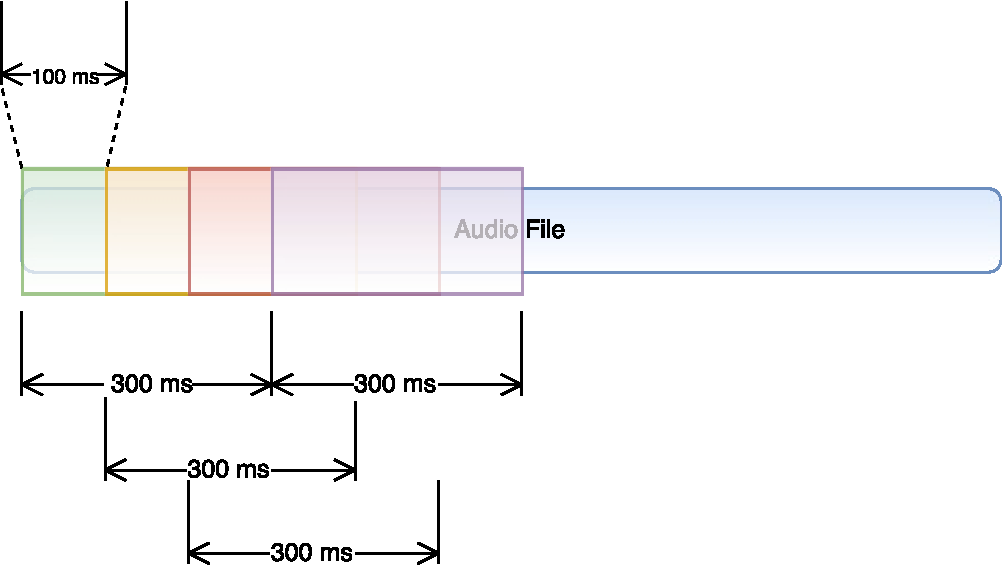
\includegraphics[scale=0.7]{OverlappingSplits300ms.pdf}
    \caption{Overlapping Segmentation}
    \label{fig:overlappingSegmentation}
\end{figure}
\end{frame}

\begin{frame}[allowframebreaks]
\frametitle{Audio Correction: Re-assembling the segments}
\begin{enumerate}
 \item Classifier gave the labels of the overlapping segments
 \item Remove the segments which were labelled as STUTTER and combine the segments labelled as NORMAL
 \item One way of assembling the segments was to append contiguous chunks together
 \begin{enumerate}
  \item This will result in sharp interjections at the point of concatenation
  \item Very artificial sounding voice
 \end{enumerate}
 \item So instead of na\"ively appending the adjacent chunks, we interpolated the audio samples between the end of the previous chunk and the beginning of the current chunk
\end{enumerate}

\begin{figure}[!ht]
    \centering
    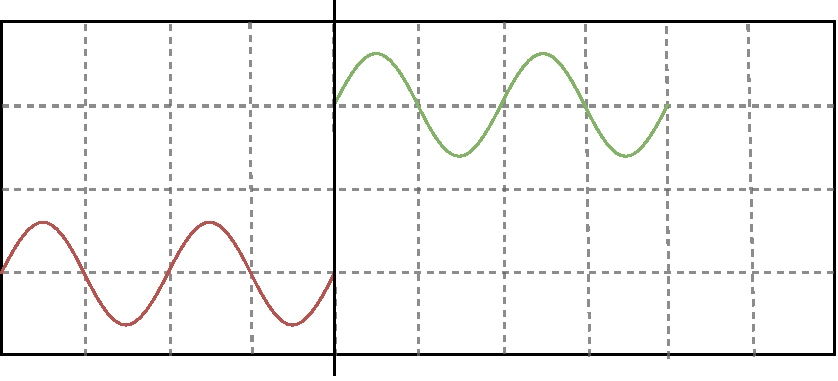
\includegraphics[scale=0.8]{NaiveReassembling.pdf}
    \caption{Na\"ive Re-assembling}
    \label{fig:naiveReassembling}
\end{figure}
\begin{figure}[!ht]
\centering
    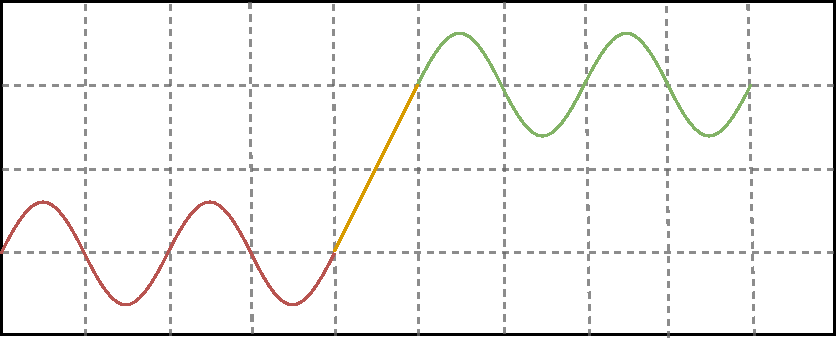
\includegraphics[scale=0.8]{SmoothReassembling.pdf}
    \caption{Smoothed Re-assembling}
    \label{fig:smoothedReassembling}
\end{figure}

\end{frame}

\begin{frame}
\frametitle{Speech-to-text}
\begin{enumerate}
 \item The UCLASS dataset \cite{uclass} is in British English
 \item We used the IBM Watson's Speech-to-text \cite{speechToText} which already has a trained model for GB English.
\end{enumerate}
\end{frame}


\begin{frame}
\frametitle{Results}
\begin{enumerate}
 \item As we can see, our model is far from perfect
 \item But we achieved some improvement over the un-modified audio files
 \item With the limited dataset available for training, we could only achieve this much accuracy
\end{enumerate}

\begin{table}[ht]
\centering
\caption{Comparison of WER of original and the corresponding corrected audio}
\label{table:werComparision}
\begin{tabular}{|l|r|r|}
\hline
\textbf{Subject}           & \multicolumn{1}{l|}{\textbf{Original (\%WER)}} & \multicolumn{1}{l|}{\textbf{Corrected (\%WER)}} \\ \hline
\textbf{M\_0017\_19y2m\_1} & 74.928\%                                       & 73.775\%                                        \\ \hline
\textbf{M\_0065\_20y1m\_1} & 125.000\%                                      & 116.429\%                                       \\ \hline
\textbf{M\_0100\_12y3m\_1} & 84.173\%                                       & 89.928\%                                        \\ \hline
\textbf{M\_1017\_11y8m\_1} & 55.396\%                                       & 48.921\%                                        \\ \hline
\textbf{M\_1017\_13y2m\_1} & 59.322\%                                       & 46.610\%                                        \\ \hline
\end{tabular}
\end{table}

\footnotesize{The source code of the project can be found at \href{https://github.com/anshulgupta0803/stutter-speech-recoginition}{https://github.com/anshulgupta0803/stutter-speech-recoginition}}
\end{frame}


\begin{frame}
\frametitle{References}
\bibliographystyle{plain}
\bibliography{references}
\end{frame}


\end{document}
